\documentclass[11pt, titlepage]{article}
\usepackage{amsmath,amsthm,amssymb}
\usepackage{hyperref, pgf, tikz}
\usepackage{fancyhdr}
\usetikzlibrary{arrows}
\usepackage[margin=1.25in]{geometry}
\usepackage{graphicx}                     
\pagestyle{fancy}
\usepackage{array}
\usepackage{indentfirst}
%\usepackage{wrapfig}

\lhead{Lab \#4}
\rhead{\thepage}
\cfoot{}

\title{Introduction to the Oscilloscope \\ \ \\ \large Lab \#4}
\author{Name: Avery Karlin \\ Partner: Kevin Yan}
\date{}
\begin{document}

\maketitle

\begin{center}
\LARGE Introduction to the Oscilloscope
\end{center}

\section*{Objective}
The objective of the lab is to learn about the oscilloscope, how to use it, and to test out using it to measure AC current.

\section*{Discussion}

Within this lab, it was first explained that the oscilloscope is based on a cathode ray tube, or an electron beam from a heated filament, firing electrons through a focus and accelerator into a fast beam, moving through parallel plates in both directions to change the location of the beam before it hits the screen. As a result, voltage of differing quantities can be applies to the plate, moving it a fixed distance from the origin. As a result, if there is a constantly increasing voltage on the horizontal plates, with the vertical plates voltage created by an outside source, it produces a graph of the voltage versus time.

\begin{figure}[h]
\centering
\hspace*{0cm}
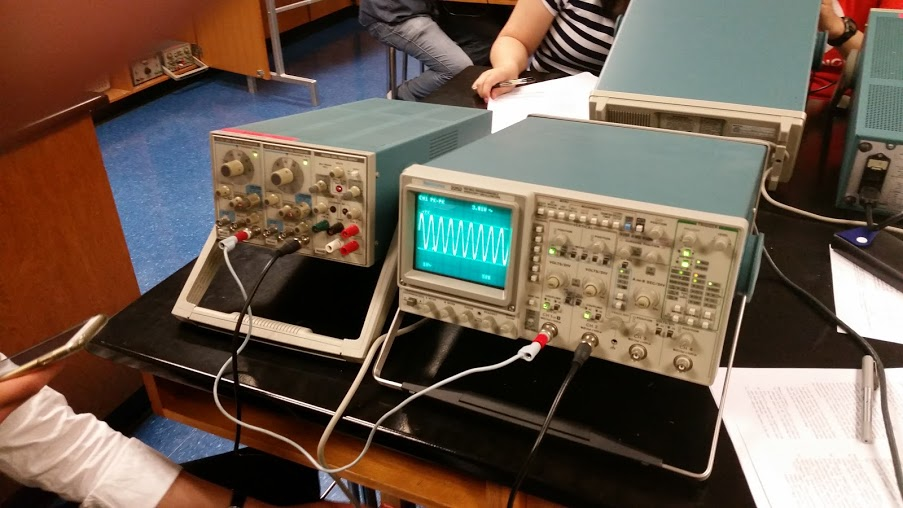
\includegraphics[scale=0.5]{lab41.jpg}
\vspace*{0cm}
\end{figure}

Using the voltmeter settings of the oscilloscope, it is able to measure the maximum voltage of an AC current, a DC current, or the difference between the maximum and minimum, recording it on the screen. Using the counter timer setting, it is able to measure the period or frequency of an AC current similarly, recording it on the screen. The volts per division and seconds per division dials are able to change the scale of the graph, with fine tuning dials attached to them to change on a smaller scale. This scale can also be used to calculate the period or frequency manually, based on the number of divisions, since the time per division is known.  There are also placement dials to adjust or move the location of the origin, to give a different view of the graph, which generally should be set up before hand.

In addition, multiple voltage sources are able to be connected to the oscilloscope, overlaid on each other based on the sources pressed. The add button allowed both to be added together, to see the beats of the combined signals. In addition, the graph can be changed from against time, to the X-Y setting, which places one signal on the X axis, the other on the Y axis, such that it can form Lissajeous figures as a result, or closed looping figures.

Finally, the AC generator is a far simpler device, allowing setting of the frequency and the amplitude of the voltage, as well as the type of wave, either jagged, square, or sine, changing the pattern within the oscilloscope itself.

\end{document}
